\documentclass[a4paper,12pt]{article}
\usepackage{graphicx}  % Do wstawiania obrazków
\usepackage{titlesec}  % Dodatkowe formatowanie tytułów
\usepackage{lmodern}   % Lepsza jakość czcionek
\usepackage{hyperref}
\usepackage{xcolor}
\usepackage{float}
\usepackage{listings}
\usepackage[polish]{babel}
\usepackage[a4paper, left=2.5cm, right=2.5cm, top=2.5cm, bottom=2.5cm]{geometry}


\usepackage[T1]{fontenc}
\lstset{
    language=Python,            % język programowania
    basicstyle=\ttfamily\footnotesize, % czcionka
    numbers=left,               % numerowanie linii po lewej stronie
    numberstyle=\tiny,          % rozmiar numerów
    stepnumber=1,               % numerowanie co 1 linię
    numbersep=5pt,              % odstęp numeru od kodu
    backgroundcolor=\color{lime}, % kolor tła
    captionpos=b,               % pozycja podpisu (b - bottom)
    breaklines=true,            % łamanie linii
    breakatwhitespace=true,     % łamanie tylko w białych znakach
}


\begin{document}

\begin{titlepage}
    \centering
    
\includegraphics[width=4cm]{logo PWr kolor pion bez tla.png}
    
    \vspace{1cm}
    {\huge Projektowanie i programowanie gier \\ Laboratorium \par}
    
    \vspace{2cm}
    {\huge\bfseries Raport\par}
    
    \vspace{2cm}
    {\Large Julia Krok 272981 \par}
    
    \vspace{2cm}
    \textbf{Prowadzący} \par
    \Large Dr inż. arch. Tomasz Zamojski
    
    \vspace{1.5cm}
    {\large marzec 2025 \par}
\end{titlepage}

\tableofcontents
\newpage
\section{Wprowadzenie}
Raport przedstawia proces tworzenia pierwszych gier komputerowych w ramach laboratorium z przedmiotu "Projektowanie i Programowanie Gier".
\\

Do tworzenia gier wykorzystywany jest silnik GODOT na licencji MIT. Gry zostaną wykonane zgodnie z instrukcjami dostępnymi na
\href{https://docs.godotengine.org/pl/4.x/getting_started}{stronie}.

\section{Pierwsza gra 2D}

\subsection{Przygotowanie projektu}
Gra polegać będzie na poruszaniu graczem tak aby unikać kolizji z przeciwnikami. Za każdą sekundę gry zostanie przyznany punkt.
\\

Na projekt składają się z elementy:
\begin{enumerate}
    \item Scena gracza --- Player
    \item Scena przeciwników --- Mob
    \item Główna scena gry --- Main
    \item HUD (ang. Heads-up Design)    
\end{enumerate}
Każdy z elementów reprezentowany jest przez węzeł (ang. Node) zawierający części z których jest złożony.\\

Podstawowe typy plików wykorzystywane przy programowaniu gry to:
\begin{enumerate}
    \item .gd --- GDScript --- Plik ze skryptami opisującymi zachowanie elementu
    \item .tscn --- PackedScene  --- Plik z obiektami zawierającymi się w scenie
\end{enumerate}

\newpage
\subsection{Utworzenie gracza}
Na początku utworzona została scena gracza jako element \textit{Area2D}. Węzeł gracza składa się z animowanego elementu graficznego reprezentującego gracza otoczonego przez dopasowany prosty kształ kolizji. 

\begin{figure}[h]
    \centering
    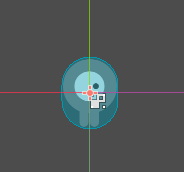
\includegraphics[width=0.4\textwidth]{player.png}
    \caption{Widok gracza.}
    \label{fig:player1}
\end{figure}

\begin{lstlisting}[language=Python]
extends Area2D
signal hit

@export var speed = 400 # How fast the player will move (pixels/sec).
var screen_size # Size of the game window.

func _ready():
	screen_size = get_viewport_rect().size
	hide()
	
func _process(delta):
	var velocity = Vector2.ZERO # The player's movement vector.
	if Input.is_action_pressed("move_right"):
		velocity.x += 1
	if Input.is_action_pressed("move_left"):
		velocity.x -= 1
	if Input.is_action_pressed("move_down"):
		velocity.y += 1
	if Input.is_action_pressed("move_up"):
		velocity.y -= 1

	if velocity.length() > 0:
		velocity = velocity.normalized() * speed
		$AnimatedSprite2D.play()
	else:
		$AnimatedSprite2D.stop()
		
	position += velocity * delta
	position = position.clamp(Vector2.ZERO, screen_size)
	
	if velocity.x != 0:
		$AnimatedSprite2D.animation = "walk"
		$AnimatedSprite2D.flip_v = false
		# See the note below about the following boolean assignment.
		$AnimatedSprite2D.flip_h = velocity.x < 0
	elif velocity.y != 0:
		$AnimatedSprite2D.animation = "up"
		$AnimatedSprite2D.flip_v = velocity.y > 0


func _on_body_entered(body: Node2D):
	hide() # Player disappears after being hit.
	hit.emit()
	# Must be deferred as we can't change physics properties on a physics callback.
	$CollisionShape2D.set_deferred("disabled", true)
	
func start(pos):
	position = pos
	show()
	$CollisionShape2D.disabled = false

\end{lstlisting}

 Zaimplementowana została obsługa zdarzeń klawiatury: naciśnięcie strzałek powoduje przesunięcie gracza w odpowiednim kierunku.
 
\begin{figure}[h]
    \centering
    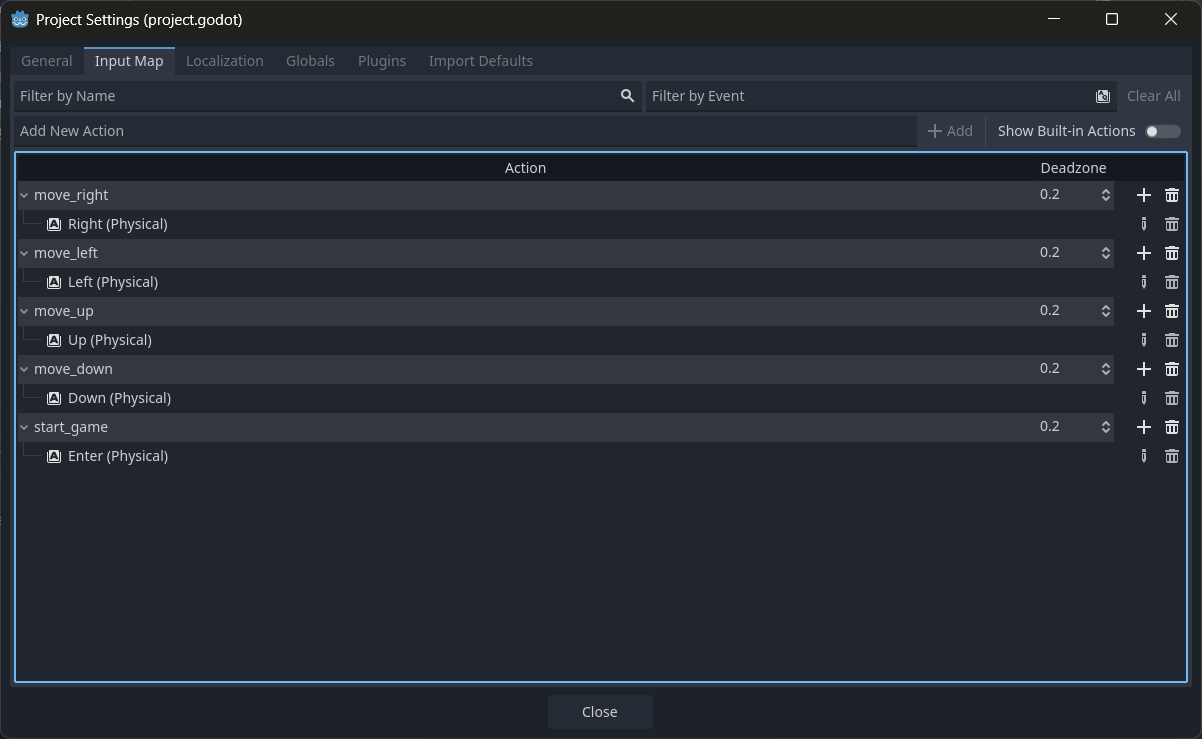
\includegraphics[width=1.0\textwidth]{Input_map.png}
    \caption{Mapa obsługi klawiatury.}
    \label{fig:player1_script}
\end{figure}

\newpage
\subsection{Utworzenie przeciwników}

Utworzenie przeciwników odbyło się w sposób analogiczny do utworzenia gracza na podstawie elementu \textit{RigidBody2D}. Istnieją trzy rodzaje przeciwników: chodzący, pływający i latający. Będą oni generowani na obrzeżach ekranu, a potem będą poruszali się po linii prostej.

\begin{lstlisting}[language=Python]
extends RigidBody2D

func _ready():
	var mob_types = Array($AnimatedSprite2D.sprite_frames.get_animation_names())
	$AnimatedSprite2D.animation = mob_types.pick_random()
	$AnimatedSprite2D.play()

func _on_visible_on_screen_notifier_2d_screen_exited():
	queue_free()
\end{lstlisting}

\begin{figure}[h]
    \centering
    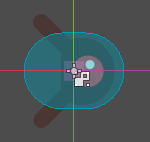
\includegraphics[width=0.4\textwidth]{mob_swim.png}
    \caption{Widok przeciwnika.}
    \label{fig:mob1}
\end{figure}

\newpage
\subsection{Utworzenie głównej sceny}

Główna scena oparta jest na podstawowym elemencie \textit{Node}. Do niej dodany zastał prostokąt o wybranym kolorze jako tło, timery oraz pliki dźwiękowe. Tutaj ustawiona jest również pozycja początkowa oraz pozycja pojawiania się przeciwników.

\begin{figure}[h]
    \centering
    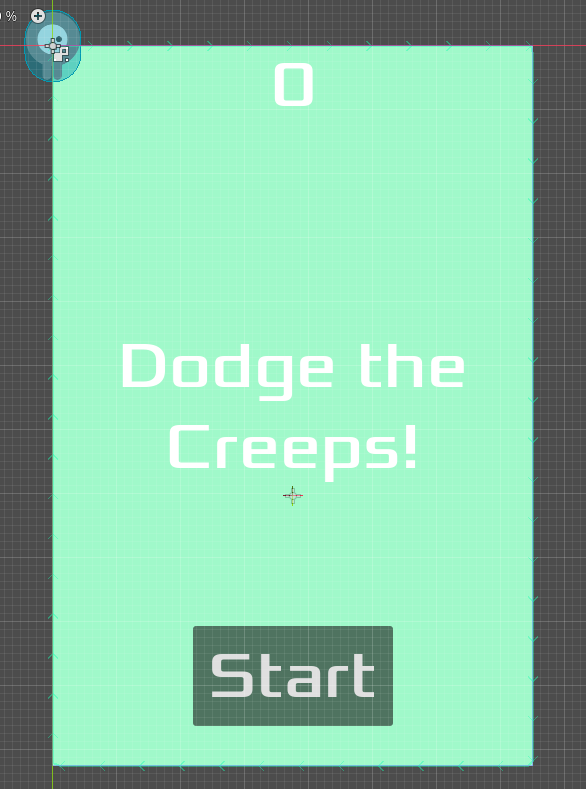
\includegraphics[width=0.5\textwidth]{main.png}
    \caption{Widok głównej sceny gry.}
    \label{fig:main1}
\end{figure}

\begin{lstlisting}[language=Python]
extends Node

@export var mob_scene: PackedScene
var score

func _ready():
	pass

func game_over() -> void:
	$ScoreTimer.stop()
	$MobTimer.stop()
	$HUD.show_game_over()
	$Music.stop()
	$DeathSound.play()

func new_game():
	score = 0
	$Player.start($StartPosition.position)
	$StartTimer.start()
	$HUD.update_score(score)
	$HUD.show_message("Get Ready")
	get_tree().call_group("mobs", "queue_free")
	$Music.play()

func _on_mob_timer_timeout() -> void:
	# Create a new instance of the Mob scene.
	var mob = mob_scene.instantiate()

	# Choose a random location on Path2D.
	var mob_spawn_location = $MobPath/MobSpawnLocation
	mob_spawn_location.progress_ratio = randf()

	# Set the mob's position to the random location.
	mob.position = mob_spawn_location.position

	# Set the mob's direction perpendicular to the path direction.
	var direction = mob_spawn_location.rotation + PI / 2

	# Add some randomness to the direction.
	direction += randf_range(-PI / 4, PI / 4)
	mob.rotation = direction

	# Choose the velocity for the mob.
	var velocity = Vector2(randf_range(150.0, 250.0), 0.0)
	mob.linear_velocity = velocity.rotated(direction)

	# Spawn the mob by adding it to the Main scene.
	add_child(mob)


func _on_score_timer_timeout() -> void:
	score += 1
	$HUD.update_score(score)


func _on_start_timer_timeout() -> void:
	$MobTimer.start()
	$ScoreTimer.start()
\end{lstlisting}

\subsection{HUD}

Na końcu dodana została też nakładka z przyciskiem "Start" oraz licznikiem punktów i wiadomością \textit{Dodge the Creeps}. Dołączony skrypt obsługuje poprawne wyświetlanie wiadomości oraz uruchomienie powiązanych liczników czasu.

\begin{lstlisting}[language=Python]
extends CanvasLayer

# Notifies `Main` node that the button has been pressed
signal start_game

func show_message(text):
	$Message.text = text
	$Message.show()
	$MessageTimer.start()
	
func show_game_over():
	show_message("Game Over")
	# Wait until the MessageTimer has counted down.
	await $MessageTimer.timeout

	$Message.text = "Dodge the Creeps!"
	$Message.show()
	# Make a one-shot timer and wait for it to finish.
	await get_tree().create_timer(1.0).timeout
	$StartButton.show()
	
func update_score(score):
	$ScoreLabel.text = str(score)

func _on_start_button_pressed() -> void:
	$StartButton.hide()
	start_game.emit()

func _on_message_timer_timeout() -> void:
	$Message.hide()
\end{lstlisting}

\begin{figure}[h]
    \centering
    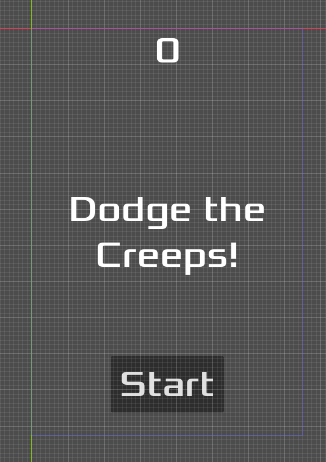
\includegraphics[width=0.5\textwidth]{HUD.png}
    \caption{HUD.}
    \label{fig:HUD1}
\end{figure}

\newpage
\subsection{Ostateczny wygląd interfejsu gry}

\begin{figure}[htb]
    \centering
    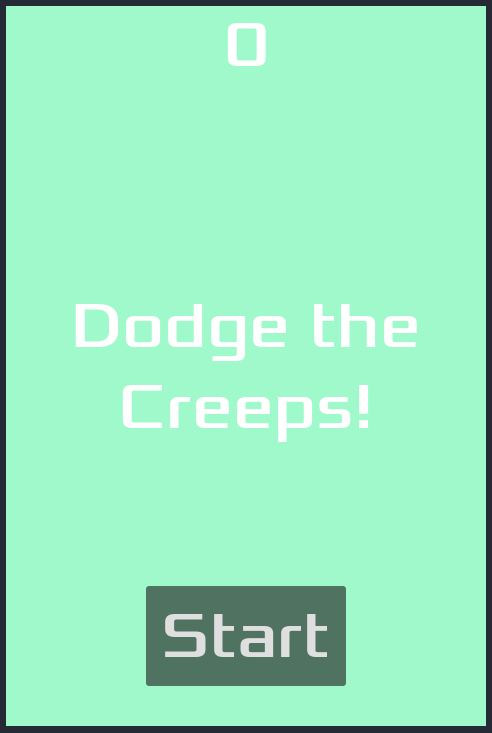
\includegraphics[width=0.33\textwidth]{begin.png}
    \caption{Widok początkowy gry.}
    \label{fig:begin1}
\end{figure}

\begin{figure}[htb]
    \centering
    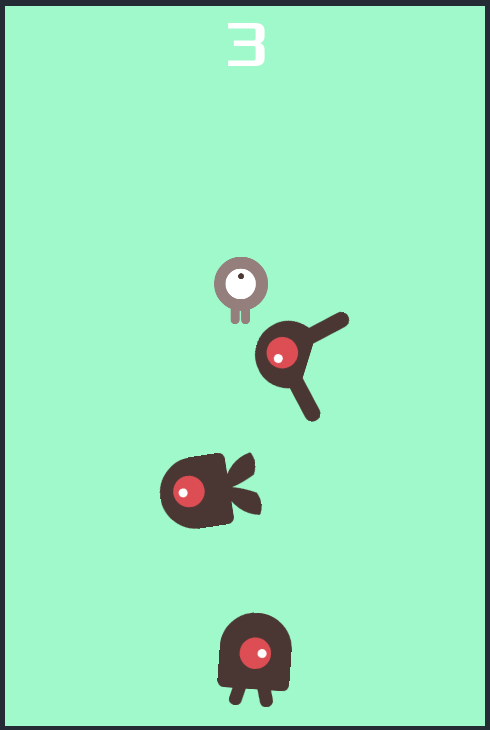
\includegraphics[width=0.33\textwidth]{play.png}
    \caption{Widok podczas gry.}
    \label{fig:play1}
\end{figure}

\begin{figure}[h]
    \centering
    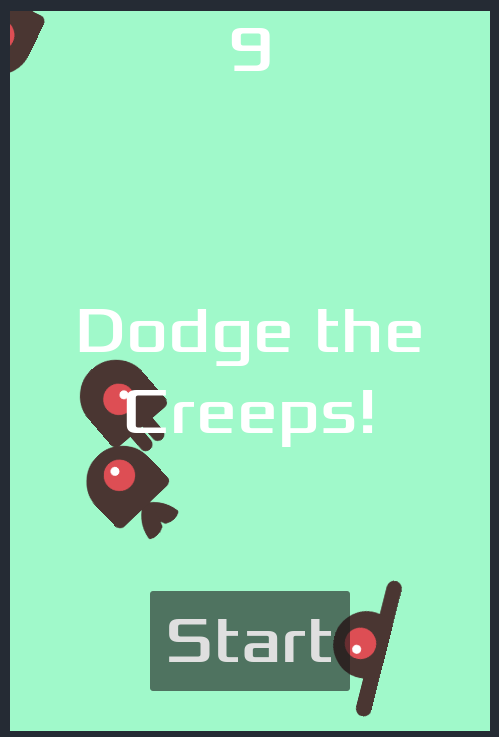
\includegraphics[width=0.33\textwidth]{end.png}
    \caption{Widok końcowy gry.}
    \label{fig:end1}
\end{figure}

\newpage
\section{Pierwsza gra 3D}

\end{document}

